\documentclass[xcolor=dvipsnames]{beamer}
\usepackage{bibentry}
\nobibliography*
\newcommand\myitembullet{{\color{blue}\usebeamertemplate{itemize
      item}\hspace{.5em}}}
\newcommand\beamerblue[1]{{\usebeamercolor[fg]{structure}#1}}
\setbeamercolor{emph}{fg=red}
\renewcommand<>{\emph}[1]{%
  {\usebeamercolor[fg]{emph}\only#2{\itshape}#1}%
}
\usepackage{pdfpages}
\usepackage{xspace}
\usepackage{stmaryrd}
\usepackage{dsfont}
\usepackage{caption}
\usepackage{csquotes}
\usepackage{mathtools}
\usepackage{tipa}
\usepackage{graphicx}
\usepackage{relsize}
\usepackage{amssymb}
\usepackage{amsmath}
\usepackage{mathabx}
\usepackage{url}
\usepackage{hyperref}
\usepackage[author=]{fixme}[2013/01/28]
\usepackage{chngpage}



\newcommand\paror{\sqsubseteq}
\newcommand\strictparor{\sqsubset}
\newcommand\nparor{\nsqsubseteq}
\newcommand\powset{\mathcal{P}}
\newcommand\all[1]{[#1]}
\newcommand\some[1]{\langle #1 \rangle}
\newcommand\lfp[2]{\mu #1 . #2}
\newcommand\gfp[2]{\nu #1 . #2}
\newcommand\nat{\mathds{N}}
\newcommand\mmeaning[1]{\llbracket #1 \rrbracket}
\newcommand\lub{\bigsqcup}
\newcommand\glb{\bigsqcap}
\newcommand\lalways{\boxvoid}
\newcommand\leventually{\lozenge}
\newcommand\lnext{\ovoid}
\newcommand\luntil{\mathcal{U}}
\newcommand\lwuntil{\mathcal{W}}
\newcommand\lrelease{\mathcal{R}}
\newcommand\trans[1]{\xrightarrow{\text{#1}}}
\newcommand\transys{\mathcal{M}}
\newcommand\valuation{\mathcal{V}}
\newcommand\game{\mathcal{G}}
\newcommand\bisim{\mathcal{R}}

\begin{document}

\title{A glimpse at the $\mu$-calculus}
\author{\small Precise Modeling and Analysis group\\University of
  Oslo\\Daniel Fava\date{\today}
}

\frame{\titlepage}

\section{Outline}
\frame{\frametitle{Roadmap}
  \begin{enumerate}
  \item Start with LTL and motivate greater expressivity
  \item Give some background: {\small Hennessy Milner Logic (HML)}
  \item Build a modest foundation for understanding fixed points
  \item $\mu$-calculus syntax, semantics, and examples
  \item Game theoretic approach to model checking the $\mu$-calculus
  \item Bisimulation
  \end{enumerate}
}

\section{Motivation}
\frame{\frametitle{Motivation}
  What do these mean?\onslide<3->{  {\color{red}Notice the recursion}}
  \begin{align*}
    \beamerblue{\lalways p} \onslide<2->{&= p \land \lnext \lalways p}\\
    \beamerblue{\leventually p} \onslide<2->{&= p \lor \lnext \leventually p}\\
    \beamerblue{p \luntil q} \onslide<2->{&= q \lor \big(p \land \lnext (p \luntil q)\big)}\\
    \beamerblue{p \lrelease q} \onslide<2->{&= (p \land q) \lor \big(q \land \lnext (p \lrelease q)\big)}
  \end{align*}
  \visible<3->{
  \begin{itemize}
  \item[] Think of $\lalways$, $\leventually$, $\luntil$,
  $\lrelease$ as special purpose recursive operators
  \item[${\color{red}\bullet}$] What if we could have more powerful
    (arbitrary) recursions?
  \end{itemize}
 }
}
% NOTE:
%% Draw the eval for always and release on the board.
%% Point out base case and inductive step.

\frame{\frametitle{Motivation}
  \beamerblue{LTL}: {\small a trace $\sigma$ or sets of traces}
  \[\mmeaning{\alpha}^{\sigma}=\{T,F\} \]
  \beamerblue{$\mu$-calculus}: {\small Labeled Transition System (LTS)
    \beamerblue{$\transys=(S,\trans{l},P_i)$}}
      \[\mmeaning{\alpha}^\transys \subseteq S \]
  \begin{enumerate}
    \item Talk about a node's direct children \onslide<2->{{\small \color{red}$\Longleftarrow$ Hennessy Milner Logic}}
    \item Talk about a node's descendants \onslide<2->{{\small \color{red}$\Longleftarrow$ Fixed points}}
  \end{enumerate}
  \includegraphics[trim={0 1cm 0 1cm},scale=0.5]{figures/lts.pdf}
}

%\section{Background}
%\frame{\frametitle{Background: Labeled Transition Systems (LTS)}
%  \begin{itemize}
%    \item \beamerblue{$\transys=(S,\trans{l},P_i)$} is a tuple called a label
%      transition system
%      \begin{itemize}
%      \item[] $S$ is a set of states, $L$ is a set of labels,
%      \item[] $\trans{l}$ are labeled transitions between states
%        ($l\in L$), and
%      \item[] $P_i \subseteq S$ is a set of states for every
%        proposition $p_i$
%      \end{itemize}
%    \item \beamerblue{$\mmeaning{\Phi}^\transys$} denotes a formula $\Phi$
%      evaluated on the LTS $\transys$
%      \begin{itemize}
%      \item[${\color{red}\bullet}$] A formula evaluates to a subset of the states:
%        $\mmeaning{\Phi}^\transys \subseteq S$
%      \end{itemize}
%  \end{itemize}
%  \onslide<2->{
%    {\centering \includegraphics[trim={0 1cm 0
%          1cm},scale=0.5]{figures/lts_hml.pdf}}
%    }
%}

\frame{\frametitle{Background: Hennessy Milner Logic {\tiny(1/3)}}
  \begin{itemize}
  \item Syntax~~~
  $\Phi ::= \color{red} tt ~|~ ff ~|~ p_i ~|~ \lnot p_i \color{black}
    ~|~ \Phi_1 \land \Phi_2 ~|~ \Phi_1 \lor \Phi_2
    ~|~ \all{a} \Phi ~|~ \some{a} \Phi
    $
  \item Semantics
  \end{itemize}
  \begin{align*}
    \mmeaning{tt}^\transys =S ~~~~~&~~~~
    \mmeaning{ff}^\transys=\emptyset\\% ~~~~~&~~~~
    \mmeaning{p_i}^\transys =P_i ~~~~~&~~~~ 
    \mmeaning{\lnot p_i}^\transys=S-P_i
  \end{align*}
  \begin{columns}[T]
    \begin{column}{.5\textwidth}
      {\centering \includegraphics[trim={0 1cm 0
            1cm},scale=0.5]{figures/lts_hml.pdf}}
    \end{column}
    \begin{column}{.5\textwidth}
      Examples:
      \begin{enumerate}
        \item $\mmeaning{tt}^\transys=\{n_1,n_2,n_3,n_4,n_5\}$
        \item $\mmeaning{p}^\transys=\{n_1,n_3,n_4\}$
      \end{enumerate}
    \end{column}
  \end{columns}
}
%% NOTES:
%% Emphasize absence of negation
%%
%% Go through examples
%%   [tt] = {n1, n2, n3, n4}
%%   [ff] = empty
%%   [p] = {n1, n3, n4}
%%   [q] = {n1, n2, n4}

\frame{\frametitle{Background: Hennessy Milner Logic {\tiny(2/3)}}
  \begin{itemize}
  \item Syntax~~~
  $\Phi ::= tt ~|~ ff ~|~ p_i ~|~ \lnot p_i
    ~|~ \color{red} \Phi_1 \land \Phi_2 ~|~ \Phi_1 \lor \Phi_2 \color{black}
    ~|~ \all{a} \Phi ~|~ \some{a} \Phi
    $
  \item Semantics
    \begin{align*}
      \mmeaning{\alpha \lor \beta}^\transys=&\mmeaning{\alpha}^\transys
      \cup \mmeaning{\beta}^\transys\\
      \mmeaning{\alpha \land \beta}^\transys=&\mmeaning{\alpha}^\transys \cap \mmeaning{\beta}^\transys
    \end{align*}
  \end{itemize}
  \begin{columns}[T]
    \begin{column}{.5\textwidth}
      {\centering \includegraphics[trim={0 1cm 0
        1cm},scale=0.5]{figures/lts_hml.pdf}}
    \end{column}
    \begin{column}{.5\textwidth}
      \vspace{10pt}
      Example:\vspace{5pt}\\
      ~~$\mmeaning{p\land q}^\transys=\{n_1,n_4\}$
    \end{column}
  \end{columns}
}

\frame{\frametitle{Background: Hennessy Milner Logic {\tiny(3/3)}}
  \begin{itemize}
  \item Syntax~~~
  $\Phi ::= tt ~|~ ff
    ~|~ p_i ~|~ \lnot p_i
    ~|~ \Phi_1 \land \Phi_2 ~|~ \Phi_1 \lor \Phi_2
    ~|~ \color{red} \all{a} \Phi ~|~ \some{a} \Phi
    $
  \item Semantics
    \begin{itemize}
      \item[$\all{a}$] All children accessible via an $a$-transition
        $\mmeaning{\all{a} \alpha}^\transys =\{s \in S ~|~ \forall t .~~ s
        \trans{a} t ~~\rightarrow t \in \mmeaning{\alpha}^\transys \}$
      \item[$\some{a}$] At least one child accessible via an
        $\mmeaning{\some{a} \alpha}^\transys =\{s \in S ~|~ \exists t .~~ s
        \trans{a} t ~~\land~~ t \in \mmeaning{\alpha}^\transys \}$
    \end{itemize}
  \end{itemize}
  \begin{columns}[T]
    \begin{column}{.5\textwidth}
      {\centering \includegraphics[trim={0 1cm 0
            1cm},scale=0.5]{figures/lts_hml.pdf}}
      \end{column}
    \begin{column}{.5\textwidth}\vspace{10pt}
      Examples:
      \begin{enumerate}
        \item $n_1 \in \mmeaning{\all{a} q}^\transys$
        \item $n_1 \notin \mmeaning{\all{a} p}^\transys$
        \item $n_1 \in \mmeaning{\some{a} p}^\transys$
      \end{enumerate}
    \end{column}
  \end{columns}
}
%% NOTE
%% Leave HML formulas up on the board, because we will use them later

\frame{\frametitle{Background: Fixed-points {\tiny(1/3)}}
  \begin{itemize}
    \item Fixed point \onslide<2->{{\color{red}~~ $f(x)=x^2+x-4$}}
    \item Monotonic function
      \onslide<2->{{\color{red}~~ $x \leq x'
        \rightarrow f(x) \leq f(x')$}}
    \item Partial order relation {\only<2>{\color{red}}$\paror$}
    \item Upper bound \onslide<2->{{\color{red}$Y \subseteq S$, $u \in S$, if
      $\forall s \in S.~ s \paror u$}}
    \item Least Upper Bound (lub)~~~ {\only<2>{\color{red}}$\lub$}
    \item Lower bound \onslide<2->{{\color{red}$Y \subseteq S$, $l~ \in S$, if
      $\forall s \in S.~ l \paror s$}}
    \item Greatest Lower Bound (glb)~~~ {\only<2>{\color{red}}$\glb$}
    \item Complete lattice \onslide<2->{{\color{red}
         $(S, \paror, \lub, \glb)$}}
    \item Boundedness of complete lattices \onslide<2->{{\color{red}~~~~~ $\lub
      \emptyset=\bot$,~~~~ $\glb \emptyset=\top$}}
  \end{itemize}
  \begin{itemize}
  \item[] \beamerblue{Tarski-Knaster theorem}
    \begin{itemize}
      \item A monotonic function $f : L \rightarrow L$ on
        a complete lattice $L$ has a \emph{greatest fixed point} (gfp)
        and a \emph{least fixed point} (lfp).
    \end{itemize}
  \end{itemize}
}
%% NOTE: A lattice is a set with a partial order and a
%% LUB and GLB defined between pairs of elements,
%% as opposed to LUB and GLB defined over subsets.
%% NOTE: Lattices in general are not necessarily bounded
%% for example: 0, 1, 2, 3 ...
%% Every pair has a LUB and a GLB
%% But if we speak of LUB of subsets, we see that LUB of the empty
%% subset does not exist.

\frame{\frametitle{Background: Fixed-points {\tiny(2/3)}}
  \vspace{-10pt}
  \begin{columns}[c]
    \hspace{-40pt}
    \begin{column}{.4\textwidth}
      \begin{itemize}
      \item Reductive {\color{red}$f(x) \paror x$}\vspace{40pt}
      \item Extensive {\color{red}$x \paror f(x)$}
      \end{itemize}
    \end{column}
    \begin{column}{.6\textwidth}
      \begin{center}
        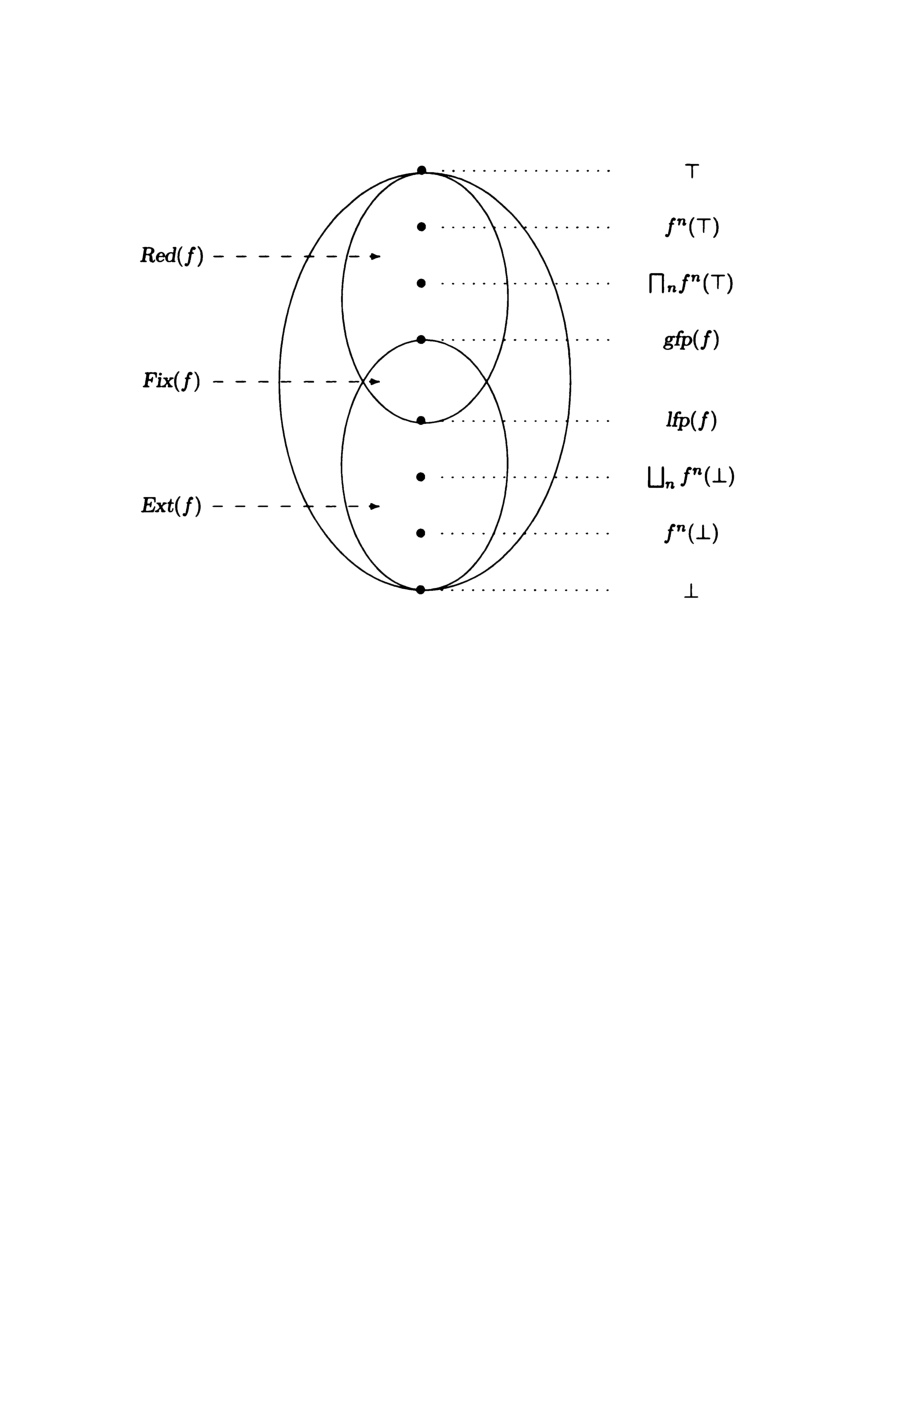
\includegraphics[scale=0.7,trim={2.4cm 13.6cm 2.9cm
            2.8cm},clip]{figures/fixed_points.pdf}
      \end{center}
    \end{column}
  \end{columns}
  \begin{itemize}
  \item[] \beamerblue{Tarski-Knaster theorem}
    \begin{itemize}
      \item A monotonic function $f : L \rightarrow L$ on
        a complete lattice $L$ has a \emph{greatest fixed point} (gfp)
        and a \emph{least fixed point} (lfp).
    \end{itemize}
  \end{itemize}
  \begin{align*}
    \textrm{gfp}(f) & = \lub \{x \in L ~|~ x \paror f(x) \} ~=~
    \lub \{Ext(f)\} \in \textrm{Fix}(f)\\
    \textrm{lfp}(f) & = \glb \{x \in L ~|~ f(x) \paror x \} ~=~
    \glb \{Red(f)\} \in \textrm{Fix}(f)
  \end{align*}
}

\frame{\frametitle{Background: Fixed-points {\tiny(3/3)}
}  \vspace{-10pt}
  \begin{columns}[c]
    \hspace{-40pt}
    \begin{column}{.4\textwidth}
      \begin{itemize}
      \item Reductive {\color{red}$f(x) \paror x$}\vspace{40pt}
      \item Extensive {\color{red}$x \paror f(x)$}
      \end{itemize}
    \end{column}
    \begin{column}{.6\textwidth}
      \begin{center}
        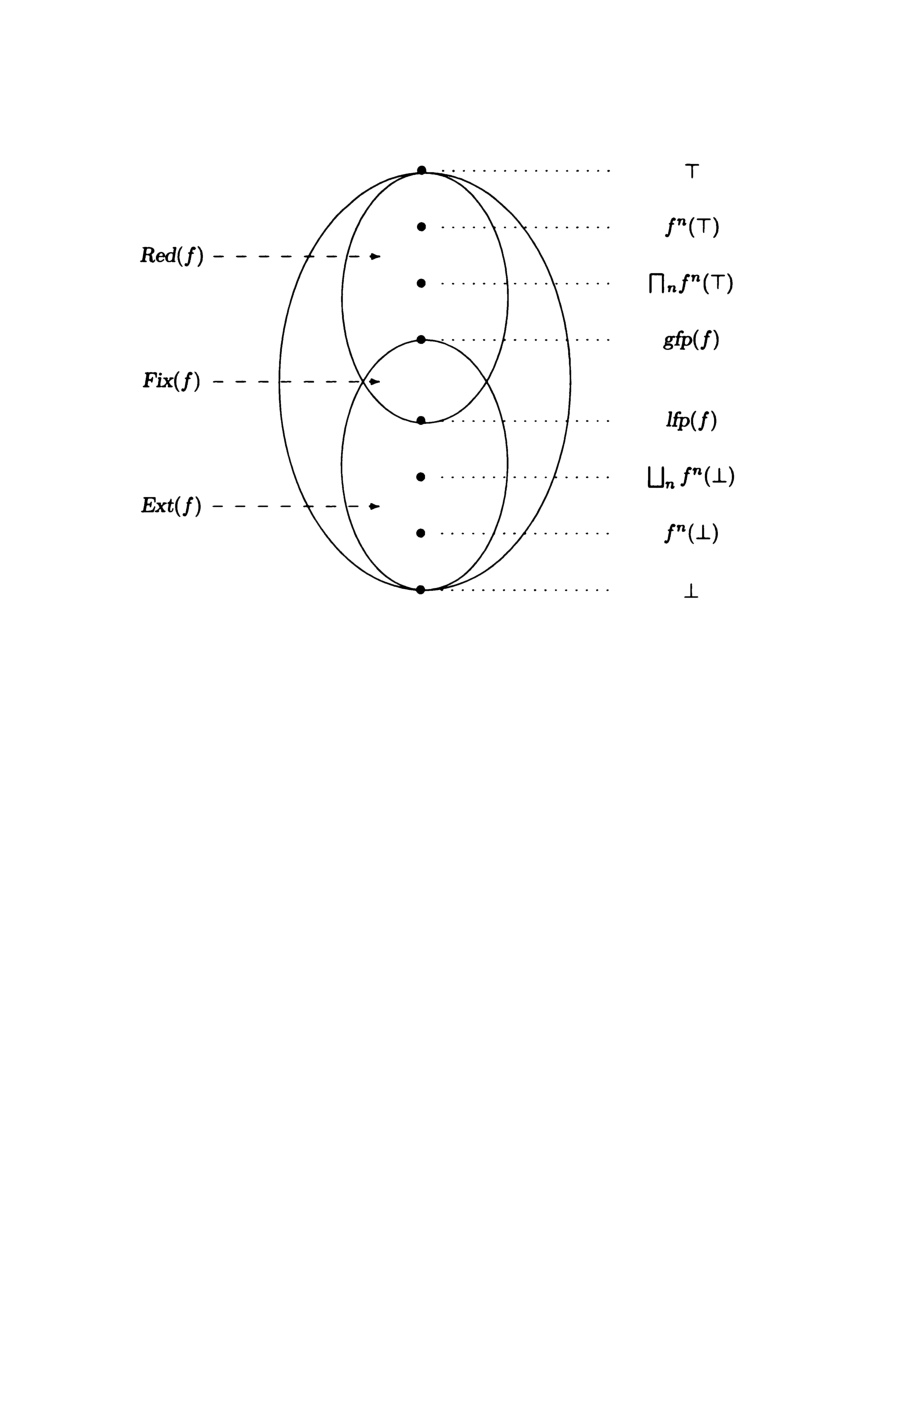
\includegraphics[scale=0.7,trim={2.4cm 13.6cm 2.9cm
            2.8cm},clip]{figures/fixed_points.pdf}
      \end{center}
    \end{column}
  \end{columns}
  \begin{itemize}
  \item[] \beamerblue{Kleene fixed-point theorem}\\
    % TODO: Formulation. How about continuity?!
    $\textrm{gfp}=f^\infty(\top)=\glb_{n \geq 0} f^n(\top)$~~~~~~~~~~
    $\textrm{lfp}=f^\infty(\bot)=\lub_{n \geq 0} f^n(\bot)$
    %\begin{align*}
    %  \textrm{gfp}&=f^\infty(\top)=\glb_{n \geq 0} f^n(\top) \\
    %  \textrm{lfp}&=f^\infty(\bot)=\lub_{n \geq 0} f^n(\bot)
    %\end{align*}
    %\begin{align*}
    %  \bot \paror f(\bot) \paror f(f(\bot)) \paror ...
    %  &\paror \textrm{lfp}(f) \\
    %  &\paror \textrm{gfp}(f) \paror... \paror f(f(\top)) \paror f(\top) \paror \top
    %\end{align*}
  \end{itemize}
}

%\frame{\frametitle{Background: Fixed-points {\tiny(3/3)}}
%  \begin{itemize}
%  \item[] \beamerblue{Kleene fixed-point theorem}
%    \begin{align*}
%      \textrm{lfp}&=f^\infty(\bot)=\lub_{n \geq 0} f^n(\bot)\\
%      \textrm{gfp}&=f^\infty(\top)=\glb_{n \geq 0} f^n(\top)
%    \end{align*}
%    \begin{align*}
%      \bot \paror f(\bot) \paror f(f(\bot)) \paror ...
%      &\paror \textrm{lfp}(f) \\
%      &\paror \textrm{gfp}(f) \paror... \paror f(f(\top)) \paror f(\top) \paror \top
%    \end{align*}
%  \end{itemize}
%  \begin{center}
%    \includegraphics[scale=0.7,trim={0cm 1.8cm 0cm
%        2.4cm},clip]{figures/kleene_1_bot.pdf}
%  \end{center}
%}

\section{$\mu$-calculus}
\frame{\frametitle{$\mu$-calculus {\tiny(1/2)}}
  \begin{itemize}
    \item Extends HML by adding variables $X, Y, Z,...$ 
  \end{itemize}
  \begin{itemize}
  \item Syntax
    \begin{itemize}
    \item Add variables and fixed point operators on top of HML
      \begin{align*}
        \Phi ::=& tt ~|~ ff ~|~ p_i ~|~ \lnot p_i
        ~|~ \Phi_1 \land \Phi_2 ~|~ \Phi_1 \lor \Phi_2
        ~|~ \all{a} \Phi ~|~ \some{a} \Phi ~|\\
             &{\color{red}X ~|~ \lfp{X}{\Phi} ~|~ \gfp{X}{\Phi}}
      \end{align*}
    \item Variable occurrences can be free, or
    \item bounded by the fixed-point operators
      \vspace{15pt}
      \item[${\color{red}\bullet}$] Note the absence of ``first class'' negation from
        the syntax
    \end{itemize}
  \end{itemize}
}

\frame{\frametitle{$\mu$-calculus {\tiny(2/2)}}
  \begin{itemize}
    \item Semantics
    \begin{itemize}
    \item Adds function from variables to sets of states called \emph{valuation}
      \[ \valuation : Var \rightarrow 2^S \]
    \item A variable occurring free is interpreted by the valuation
      \[ \mmeaning{X}^\transys_\valuation = \valuation(X) \]
    \end{itemize}
    \begin{itemize}
    \item Fixed-points are defined according to Tarski-Knaster
      theorem
      \begin{align*}
        \mmeaning{\lfp{X}{\alpha}}^\transys_\valuation
        &=\glb\{S'\subseteq S~|~
        \mmeaning{\alpha}^\transys_{\valuation[S'/X]} \subseteq
        S' \}&\textrm{(lfp)}\\
        &=\glb\{S'\subseteq S~|~
        f(S') \subseteq S' \}&\\
        \mmeaning{\gfp{X}{\alpha}}^\transys_\valuation&=\lub\{S'
        \subseteq S~|~ S' \subseteq
        \mmeaning{\alpha}^\transys_{\valuation[S'/X]}\}&\textrm{(gfp)}\\
        &=\lub\{S' \subseteq S~|~ S' \subseteq f(S') \}&
      \end{align*}
      ~~~~~~~where $f(S')=\mmeaning{\alpha}^\transys_{\valuation[S'/X]}$
    \end{itemize}
  \end{itemize}
  \begin{itemize}
  \item[${\color{red}\bullet}$] Tarski-Knaster doesn't help us compute FPs
    \begin{itemize}
    \item[] It only guarantees their existence
    \end{itemize}
  \item[${\color{red}\bullet}$] We will use Kleene's FP theorem for computing FPs
  \end{itemize}
}

\frame{\frametitle{$\mu$-calculus: Example {\tiny(1/3)}}
  \beamerblue{$\lfp{X}{\all{a}X}$} represent states with no infinite sequences of $a$-transitions
  \begin{align*}
    \lfp{{\color{red}^0}X}{\all{a}X} &= {\color{red}\emptyset} ~~~~~~ \textrm{false} \\
    \lfp{{\color{red}^1}X}{\all{a}X} &= \all{a} \emptyset \\
    &= \{s \in S ~|~ \forall t.~ s \trans{a} t \rightarrow t \vDash
    \emptyset \} \\
    & \textrm{\small since no $t$ satisfies $\emptyset$, the right hand
      side (RHS) of $\rightarrow$ is false;} \\
    & \textrm{\small thus the left hand side (LHS) of $\rightarrow$ cannot be
      true.} \\
    & \textrm{\small This represents states with no outgoing $a$-transitions} \\
    \lfp{{\color{red}^2}X}{\all{a}X} &= \all{a} T \\
    & \textrm{\small where $T=\lfp{^1X}{\all{a}X}$ are states with
      no outgoing $a$-transitions}\\
    & \textrm{\small Thus $\mu^2$ means states with no $aa$-paths}
  \end{align*}
}

\frame{\frametitle{$\mu$-calculus: Example {\tiny(2/3)}}
\beamerblue{$\gfp{X}{p \land \all{a} X}$} is informally analogous
to LTL $\lalways p$
\begin{align*}
\gfp{{\color{red}^0}X}{p \land \all{a} X} &= {\color{red}S} ~~~~~~ \textrm{true} \\
\gfp{{\color{red}^1}X}{p \land \all{a} X} &= p \land \all{a} S\\
& \textrm{\small Intersection between all nodes satisfying $p$ (LHS
  of $\land$)}\\
& \textrm{\small and all nodes (RHS of $\land$)}\\
\gfp{{\color{red}^2}X}{p \land \all{a} X} &= p \land \all{a} T\\
& \textrm{\small Where $T=\gfp{^1X}{p \land \all{a} X}$ are all nodes that satisfy $p$}\\
& \textrm{\small Thus $\mu^2$ is the intersection between all nodes that satisfy
  $p$}\\
& \textrm{\small and all nodes that have an outgoing edge labeled $a$}\\
& \textrm{\small to a node that satisfies $p$}
\end{align*}
All nodes that satisfy $p$ and whose descendants that are reachable
through $a$-transitions also satisfy $p$.
}
%% NOTE:
%% We say ``informally analogous'' because LTL is a logic on traces
%% while mu-calc is a logic on transition systems.  So, comparing them
%% is a bit like comparing apples to oranges.

\frame{\frametitle{$\mu$-calculus: Example {\tiny(3/3)}}
\beamerblue{$\lfp{X}{p \lor (\some{a} True \land \all{a} X)}$} is
informally analogous to LTL $\leventually p$
\begin{align*}
\lfp{{\color{red}^0}X}{p & \lor (\some{a} True \land \all{a} X)} = {\color{red}\emptyset} \\
\lfp{{\color{red}^1}X}{p & \lor (\some{a} True \land \all{a} \emptyset)} = 
p \lor (\some{a} True \land \all{a} \emptyset)\\
  & \textrm{\small $\some{a} True$ is the set of states with an outer
  $a$-transition}\\
  & \textrm{\small $\all{a} \emptyset$ is the set of states with no outgoing
  $a$-transition}\\
  & \textrm{\small Therefore, intersection $\land$ is empty}\\
  & \textrm{\small and the formula boils down to the set of states
  satisfying $p$}\\
\lfp{{\color{red}^2}X}{p & \lor (\some{a} True \land \all{a} T)} = 
p \lor (\some{a} True \land \all{a} T)\\
& \textrm{\small where $T=\mu{^1}$ which means nodes satisfying $p$ }\\
& \textrm{\small $\all{a} T$ are nodes whose children reachable via
  $a$-transitions satisfy $p$ }
\end{align*}
Thus either $p$ is satisfied, or it is satisfied
via a node reachable through an $a$-transitions, or via an
$aa$-transition, or via an $a^n$-transition.
}

\frame{\frametitle{Note}
  \begin{itemize}
    \item Increasing complexity with alternation of fixed point types
      \begin{itemize}
      \item With one fix-point we talk about termination properties
      \item With two fix-points we can write fairness formulas
      \end{itemize}
    %\item Hard to understand what TODO means
  \end{itemize}
}

\frame{\frametitle{Model checking via parity games {\tiny(1/5)}}
 \begin{center}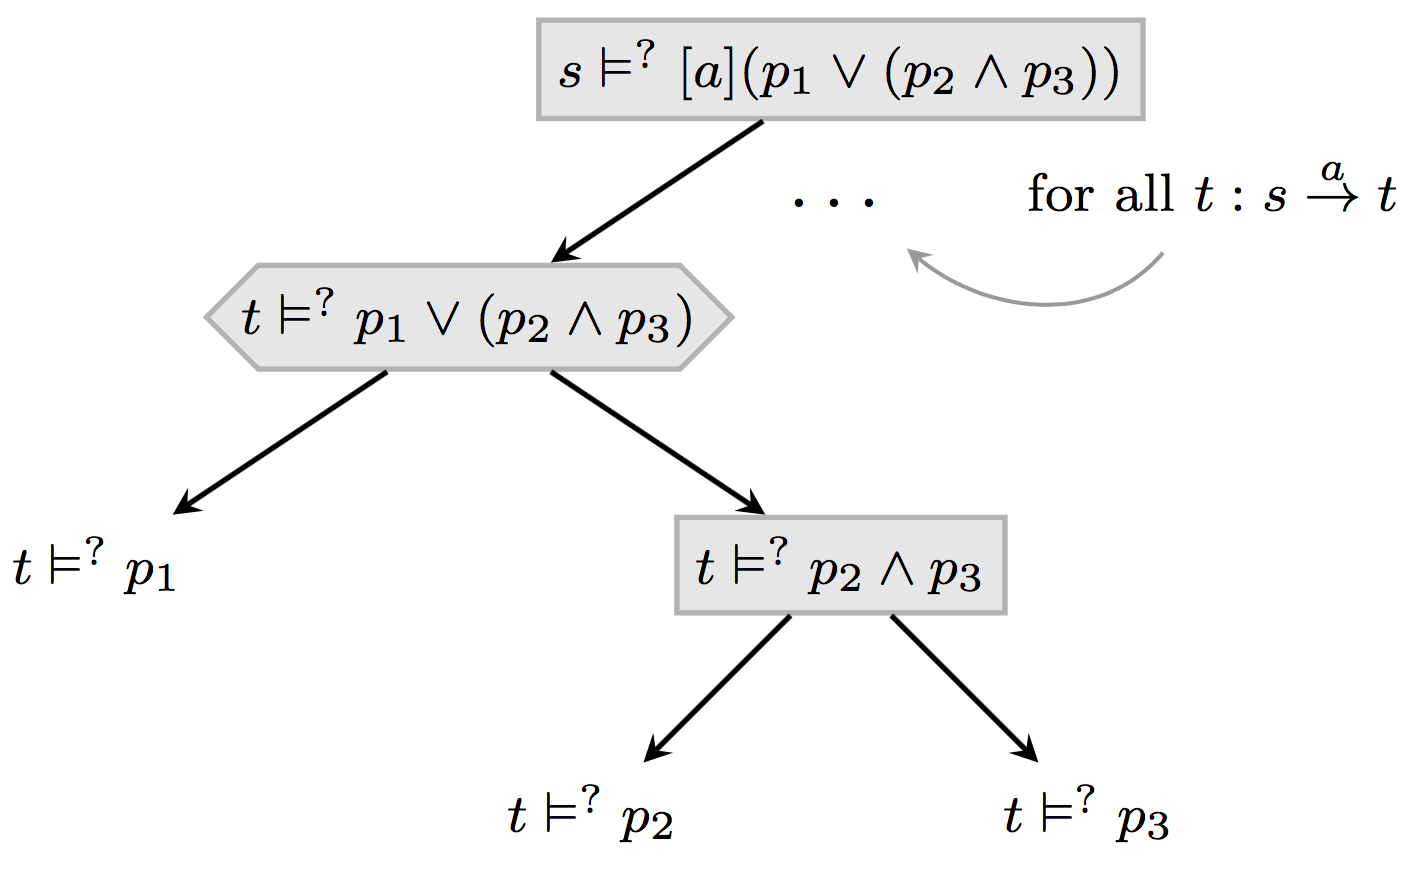
\includegraphics[scale=0.16]{figures/example.png}\end{center}
 \vspace{-10pt}
 \begin{itemize}
 \item[Adam] pick $t$ from $s \trans{a} t$ such that $t \nvDash (p_1
   \lor (p_2 \land p3)$
 \item[Eve] reply by showing that either $t \vDash p_1$ or that
   $t \vDash p_2$ and $t \vDash p_3$.
 \end{itemize}
}

\frame{\frametitle{Model checking via parity games {\tiny(2/5)}}
  \begin{definition}[Game]
    A game is a triple $G = (V, T, Acc)$ where
    \begin{enumerate}
    \item $V$ are \emph{nodes} partitioned between two players, Adam
      and Eve,\\ $V=V_A \cup V_E$ and $V_A \cap V_E = \emptyset$,
    \item $T \subseteq V \times V$ is a \emph{transition relation} determining
      the possible successors of each node, and
    \item $Acc \subseteq V^\omega$ is a set defining the \emph{winning
      condition}
    \end{enumerate}
  \end{definition}
  \begin{itemize}
    \item It is Adam's turn if $v \in V_A$, otherwise $v \in V_E$ and
      it is Eve's
    \item The player who cannot make a move loses
    \item If a play is infinite, $v_0v_1...$, then Eve wins if
      $v_0v_1... \in Acc$
  \end{itemize}
}

\frame{\frametitle{Model checking via parity games {\tiny(3/5)}}
  \begin{theorem}[Reducing model-checking to parity games]
    Let $\game(\transys, \alpha)$ denote a game constructed from the
    labeled transition system $\transys$ and the $\mu$-calculus formula
    $\alpha$.\\
    For every sentence $\alpha$, transition system $\transys$, and initial
    state $s$, then $\transys, s \vDash \alpha$ iff Eve has a winning
    strategy for the position $(s,\alpha)$ in $\game(\transys, \alpha)$.
  \end{theorem}
}

\frame{\frametitle{Model checking via parity games {\tiny(4/5)}}
  Define $\game(\transys,\alpha)$ inductively on the syntax of
  $\alpha$
  \begin{itemize}
    {\small
      \item Create node $(s,\beta)$ for every state $s$ of $\transys$
        and every formula $\beta$ in the closure of $\alpha$ {\tiny (similar
        to the automata based LTL model checking construction we have seen)}
      \item Recall that Eve's goal is to show that a formula holds, and that\\
        the player who can't make a move loses
    }
  \end{itemize}
  %\vspace{7pt}
  {\small
  \hskip-1.0cm\begin{tabular}{rl}
    \beamerblue{$(s,p)$}
      & Eve wins if $p$ holds in $s$, that is $s \vDash p$\\
      & Thus assign $(s,p)$ to Adam and we put no transitions from it
    \vspace{7pt}\\
    \beamerblue{$(s, \lnot p)$}
      & Same as $(s,p)$ but reversing Adam and Eve's roles 
    \vspace{7pt}\\
    \beamerblue{$(s, \some{a}\beta)$}
      & Connect to $(t, \beta)$ for all $t$ such
    that $s \trans{a} t$ and \\
    \beamerblue{$(s, \all{a}\beta)$}
      & assign $(s, \all{a} \beta)$ to Adam and 
      $(s, \some{a} \beta)$ to Eve
    \vspace{7pt}\\
    \beamerblue{$(s,\lfp{X}{\beta(X))}$}
      & Connect to $(s,\beta(\lfp{X}{\beta(X))})$ and to
      $(s,\beta(\gfp{X}{\beta(X))})$\\
    \beamerblue{$(s,\gfp{X}{\beta(X)})$}
      & This corresponds to the intuition that a fixed-point\\
      & is equivalent to its unfolding.
  \end{tabular}
\begin{align*}%\label{eq:unfold}
\mmeaning{\lfp{X}{\alpha}}^\transys_\valuation &=
\mmeaning{\alpha[\lfp{X}{\alpha} / X]}^\transys_\valuation\\
\mmeaning{\gfp{X}{\alpha}}^\transys_\valuation &=
\mmeaning{\alpha[\gfp{X}{\alpha} / X]}^\transys_\valuation
\end{align*}
  }
}

\frame{\frametitle{Model checking via parity games {\tiny(5/5)}}
  \begin{itemize}
    \item How to define $Acc$ and the \emph{parity winning
      condition}
      \begin{itemize}
        \item[] See \cite{bradfield2015mu}
      \end{itemize}
  \end{itemize}
  \begin{itemize}
    \item Model checking $\transys \vDash \alpha$
      \begin{itemize}
        \item[] Use algorithm for determining winner of parity game\\
          once $\game(\transys,\alpha)$ has been created
      \end{itemize}
  \end{itemize}
}
%% 
%%

\section{Bisimulation}
\frame{\frametitle{Bisimulation {\tiny(1/3)}}
  \begin{itemize}
    \item Equivalence between systems
    \begin{itemize}
    \item Preserves compositionality
      \begin{itemize}
      \item Programs as functions (denotational semantics)
        \begin{align*}
          \span x:=2 ~~~~~~ \textrm{and}~~~~~~ x:=1;~ x:=x+1 \\
          x:=2 ~||~ x:=2 ~~~\textrm{versus}~~~ x:=2 ~||~ x:=1;~ x:=x+1
        \end{align*}
      \item Language acceptance (trace equivalence)
      \end{itemize}
  \end{itemize}
    \end{itemize}\vspace{-0.5cm}
    \begin{columns}[c]
      \hspace{-1.8cm}
      \begin{column}{.5\textwidth}
        \includegraphics[scale=0.5]{figures/trace_eq_1.pdf}
      \end{column}
      \begin{column}{.5\textwidth}
        \includegraphics[scale=0.5]{figures/trace_eq_2.pdf}
      \end{column}
    \end{columns}
}

\section{Bisimulation}
\frame{\frametitle{Bisimulation {\tiny(2/3)}}
  \begin{itemize}
    \item Equivalence between systems
      \begin{itemize}
        \item Not overly strong as graph isomorphism
      \end{itemize}
  \end{itemize}
  \includegraphics[scale=0.6]{figures/iso_1.pdf}
  \includegraphics[scale=0.6]{figures/iso_2.pdf}
}

\frame{\frametitle{Bisimulation {\tiny(3/3)}}
  \begin{definition}[Bisimulation]
    Bisimulation is a symmetric relation $\bisim$ on the states of an
    LTS such that whenever $P ~\bisim~ Q$, for all $t$ we have:
    \begin{itemize}
      {\small
    \item for all $P'$ which $P \trans{t} P'$, there is $Q'$ such that $Q
      \trans{t} Q'$ and $P' ~\bisim~ Q'$
    %\item the converse, on the transitions emanating from Q, i.e., for all
    %  $Q'$ with $Q \trans{t} Q'$, there is $P'$ such that $P \trans{t} P'$
    %  and $P' ~\bisim~ Q$
      }
    \end{itemize}
  \end{definition}
  \begin{definition}[Logic equivalence]
    Two statements are logically equivalent if they have the same
    truth value in every model
  \end{definition}
  \begin{center}
  \begin{tabular}{rl}
    logic & logic equivalence\\
    \hline
    LTL & trace equivalence \\
    HML, $\mu$-calculus, CTL & bisimilarity \\
  \end{tabular}
  \end{center}
  %\begin{itemize}
  %  \item Has also been used to reduce state space
  %    \begin{itemize}
  %      \item Model minimization
  %    \end{itemize}
  %\end{itemize}
}

\frame{\frametitle{References}
\setbeamerfont{bibliography item}{size=\footnotesize}
\setbeamerfont{bibliography entry author}{size=\footnotesize}
\setbeamerfont{bibliography entry title}{size=\footnotesize}
\setbeamerfont{bibliography entry location}{size=\footnotesize}
\setbeamerfont{bibliography entry note}{size=\footnotesize}
  \begin{itemize}
    \item Lattice and fixed points
      \begin{itemize}
        \item \bibentry{nielson2015principles}
        \item \bibentry{davey2002introduction}
      \end{itemize}
    \item $\mu$-calculus and model checking
      \begin{itemize}
        \item \bibentry{bradfield2015mu}
        \item \bibentry{cleaveland1990tableau}
          \end{itemize}
    \item Bisimulation
      \begin{itemize}
        \item \bibentry{sangiorgi2012introduction}
      \end{itemize}
  \end{itemize}
  \bibliographystyle{apalike}
  \nobibliography{main}
}

\end{document}
